%   \input{header_link}
%   \begin{document}
     		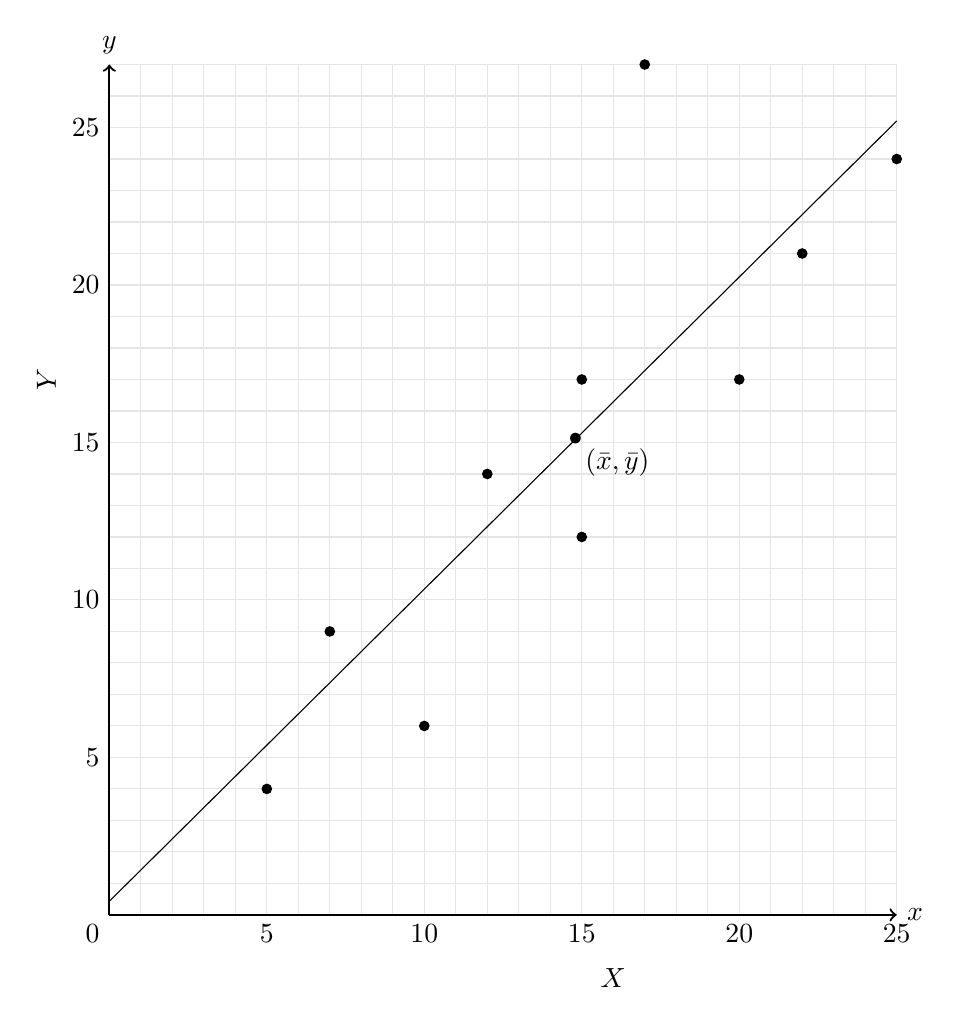
\begin{tikzpicture}[scale=0.4]
     		\newcommand{\setI}
     		{(5,4)(10,6)(7,9)(15,12)(17,27)(12,14)(20,17)(25,24)(22,21)(15,17)}
     		\draw[color=gray!20] (0,27) grid (25,0);
     		\draw[->,thick] (0,0)--(0,27) node[above]{$y$};
     		\draw[->,thick] (0,0)--(25,0) node[right]{$x$};
     		\foreach \y in {5,10,...,25} \draw(0,\y)node[left]{$\y$};
     		\foreach \x in {5,10,...,25} \draw (\x,0) node[below]{$\x$};
     		\draw (16,-2) node{$X$};
     		\draw (-2,17) node[rotate=90]{$Y$};
		\draw plot[only marks, mark=*,mark size=1.5mm] coordinates {\setI};
		\node[below left] at (0,0) {$0$};
		\node at (14.8,15.1) {$\bullet$};
		\node[below right] at (14.8,15.1) {$(\bar{x},\bar{y})$};
		\draw[domain=0:25,samples=100] plot ({\x},{0.991*\x+0.434});
		\end{tikzpicture}
%  \end{document}
